% Options for packages loaded elsewhere
\PassOptionsToPackage{unicode}{hyperref}
\PassOptionsToPackage{hyphens}{url}
%
\documentclass[
  10pt,
  english,
  doc,floatsintext]{apa6}

\usepackage{graphicx}
\makeatletter
\def\maxwidth{\ifdim\Gin@nat@width>\linewidth\linewidth\else\Gin@nat@width\fi}
\def\maxheight{\ifdim\Gin@nat@height>\textheight\textheight\else\Gin@nat@height\fi}
\makeatother
% Scale images if necessary, so that they will not overflow the page
% margins by default, and it is still possible to overwrite the defaults
% using explicit options in \includegraphics[width, height, ...]{}
\setkeys{Gin}{width=\maxwidth,height=\maxheight,keepaspectratio}
% Set default figure placement to htbp
\makeatletter
\def\fps@figure{htbp}
\makeatother
\setlength{\emergencystretch}{3em} % prevent overfull lines
\providecommand{\tightlist}{%
  \setlength{\itemsep}{0pt}\setlength{\parskip}{0pt}}
\setcounter{secnumdepth}{5}
% Make \paragraph and \subparagraph free-standing
\ifx\paragraph\undefined\else
  \let\oldparagraph\paragraph
  \renewcommand{\paragraph}[1]{\oldparagraph{#1}\mbox{}}
\fi
\ifx\subparagraph\undefined\else
  \let\oldsubparagraph\subparagraph
  \renewcommand{\subparagraph}[1]{\oldsubparagraph{#1}\mbox{}}
\fi

%\usepackage[utf8x]{inputenc}
\usepackage{amsmath}
\usepackage{amsthm}
\usepackage{graphicx}
\usepackage[colorinlistoftodos]{todonotes}

\let\B\relax 

\let\T\relax

\usepackage{gb4e}
\exewidth{(\thexnumi)} %ex number no indent setting
\let\eachwordone=\textit %first line italic
\noautomath

\usepackage[linguistics,edges]{forest} 
\forestset{
ned/.style={%
    for tree={calign=fixed edge angles},
    delay={%
      where content={}{%
        shape=coordinate,
        for nodewalk={%
          Nodewalk={%
            on invalid=fake,
          }{%
            parent,
          }{%
            for children={anchor=north},
          }
        }{},
      }{},
    },
},
fned/.style={
        delay={where content={}{shape=coordinate,
              for siblings={anchor=north}}{}},
		for tree={s sep=4mm}},
}


%\usepackage{leipzig}
%\makeglossaries


\usepackage{hyperref}
\hypersetup{colorlinks = true, linkcolor = blue, citecolor = blue, urlcolor = blue}
\usepackage{multicol}

\usepackage{listings}
\lstloadlanguages{R}
% Manuscript styling
\usepackage{upgreek}
\captionsetup{font=singlespacing,justification=justified}

% Table formatting
\usepackage{longtable}
\usepackage{lscape}
% \usepackage[counterclockwise]{rotating}   % Landscape page setup for large tables
\usepackage{multirow}		% Table styling
\usepackage{tabularx}		% Control Column width
\usepackage[flushleft]{threeparttable}	% Allows for three part tables with a specified notes section
\usepackage{threeparttablex}            % Lets threeparttable work with longtable

% Create new environments so endfloat can handle them
% \newenvironment{ltable}
%   {\begin{landscape}\begin{center}\begin{threeparttable}}
%   {\end{threeparttable}\end{center}\end{landscape}}
\newenvironment{lltable}{\begin{landscape}\begin{center}\begin{ThreePartTable}}{\end{ThreePartTable}\end{center}\end{landscape}}

% Enables adjusting longtable caption width to table width
% Solution found at http://golatex.de/longtable-mit-caption-so-breit-wie-die-tabelle-t15767.html
\makeatletter
\newcommand\LastLTentrywidth{1em}
\newlength\longtablewidth
\setlength{\longtablewidth}{1in}
\newcommand{\getlongtablewidth}{\begingroup \ifcsname LT@\roman{LT@tables}\endcsname \global\longtablewidth=0pt \renewcommand{\LT@entry}[2]{\global\advance\longtablewidth by ##2\relax\gdef\LastLTentrywidth{##2}}\@nameuse{LT@\roman{LT@tables}} \fi \endgroup}

% \setlength{\parindent}{0.5in}
% \setlength{\parskip}{0pt plus 0pt minus 0pt}

% Overwrite redefinition of paragraph and subparagraph by the default LaTeX template
% See https://github.com/crsh/papaja/issues/292
\makeatletter
\renewcommand{\paragraph}{\@startsection{paragraph}{4}{\parindent}%
  {0\baselineskip \@plus 0.2ex \@minus 0.2ex}%
  {-1em}%
  {\normalfont\normalsize\bfseries\itshape\typesectitle}}

\renewcommand{\subparagraph}[1]{\@startsection{subparagraph}{5}{1em}%
  {0\baselineskip \@plus 0.2ex \@minus 0.2ex}%
  {-\z@\relax}%
  {\normalfont\normalsize\itshape\hspace{\parindent}{#1}\textit{\addperi}}{\relax}}
\makeatother

% \usepackage{etoolbox}
\makeatletter
\patchcmd{\HyOrg@maketitle}
  {\section{\normalfont\normalsize\abstractname}}
  {\section*{\normalfont\normalsize\abstractname}}
  {}{\typeout{Failed to patch abstract.}}
\patchcmd{\HyOrg@maketitle}
  {\section{\protect\normalfont{\@title}}}
  {\section*{\protect\normalfont{\@title}}}
  {}{\typeout{Failed to patch title.}}
\makeatother
\shorttitle{current thesis draft}
\usepackage{csquotes}
\geometry{left=1in}


\geometry{right=1in}


\geometry{top=1in}


\geometry{bottom=1in}


\ifxetex
  % Load polyglossia as late as possible: uses bidi with RTL langages (e.g. Hebrew, Arabic)
  \usepackage{polyglossia}
  \setmainlanguage[]{english}
\else
  \usepackage[shorthands=off,main=english]{babel}
\fi
\ifluatex
  \usepackage{selnolig}  % disable illegal ligatures
\fi
\newlength{\cslhangindent}
\setlength{\cslhangindent}{1.5em}
\newlength{\csllabelwidth}
\setlength{\csllabelwidth}{3em}
\newenvironment{CSLReferences}[2] % #1 hanging-ident, #2 entry spacing
 {% don't indent paragraphs
  \setlength{\parindent}{0pt}
  % turn on hanging indent if param 1 is 1
  \ifodd #1 \everypar{\setlength{\hangindent}{\cslhangindent}}\ignorespaces\fi
  % set entry spacing
  \ifnum #2 > 0
  \setlength{\parskip}{#2\baselineskip}
  \fi
 }%
 {}
\usepackage{calc}
\newcommand{\CSLBlock}[1]{#1\hfill\break}
\newcommand{\CSLLeftMargin}[1]{\parbox[t]{\csllabelwidth}{#1}}
\newcommand{\CSLRightInline}[1]{\parbox[t]{\linewidth - \csllabelwidth}{#1}\break}
\newcommand{\CSLIndent}[1]{\hspace{\cslhangindent}#1}

\title{Agreement Attraction in Turkish: Effects of Bias}
\author{Utku Türk\textsuperscript{1}}
\date{}


\authornote{

Correspondence concerning this article should be addressed to Utku Türk, JF Building, No:314. E-mail: \href{mailto:utku.turk@boun.edu.tr}{\nolinkurl{utku.turk@boun.edu.tr}}

}

\affiliation{\vspace{0.5cm}\textsuperscript{1} Boğaziçi University}

\begin{document}
\maketitle

\hypertarget{summary}{%
\section*{Summary}\label{summary}}
\addcontentsline{toc}{section}{Summary}

\begin{itemize}
\item
  This file includes:

  \begin{itemize}
  \tightlist
  \item
    Tentative plannng for the thesis.
  \item
    Descriptive Stats about the experiments.
  \item
    Details (Material, Procedure, Participants) about the experiments.
  \item
    2 maximal models for Exp1 (Ungrammatical Bias) data.

    \begin{itemize}
    \tightlist
    \item
      Model 1 is a simple model with two (gram x attractor numb) predictors and by subject and by item slopes
    \item
      Model 2 only includes a predictor that is based on effect sizes of participants.
    \end{itemize}
  \item
    Information about what is going on bias-wise.
  \item
    Descriptive Stats with participants grouped according to their bias.
  \item
    Maximal modelling of all data with predictors of grammaticality, number of plural, categorical bias of the participant, and intended bias of the participants.
  \end{itemize}
\end{itemize}

\hypertarget{intro}{%
\section{Chapter 1: Introduction}\label{intro}}

\begin{itemize}
\tightlist
\item
  Aim and outline of the thesis.
\item
  Scope of the thesis.
\item
  Conventions used in the thesis.
\item
  Statistical Interference (talk about bayes, brms, ROPE (Region of Practical Equivalence), priors)
\item
  Organizaion of the thesis.
\end{itemize}

\hypertarget{aa}{%
\section{Chapter 2: Number Agreement Attraction}\label{aa}}

\begin{itemize}
\item
  Accounts of agreement attraction

  \begin{itemize}
  \tightlist
  \item
    Representational Accounts: Eberhard
  \item
    Retrieval accounts: Wagers
  \item
    Probabilistic Accounts: Gibson
  \end{itemize}
\item
  Studies of Number Agreement Attraction

  \begin{itemize}
  \tightlist
  \item
    Production
  \item
    Comprehension
  \end{itemize}
\item
  Number Agreement Attraction in Turkish
\end{itemize}

\hypertarget{chapter-3-plural-agreement-in-turkish}{%
\section{Chapter 3: Plural Agreement in Turkish}\label{chapter-3-plural-agreement-in-turkish}}

\begin{itemize}
\tightlist
\item
  Explanation of morphology
\item
  possibility to not mark it.
\item
  honorific aspect of it.
\end{itemize}

\hypertarget{bias}{%
\section{Chapter 4: Bias}\label{bias}}

\begin{itemize}
\tightlist
\item
  Bias according to Signal Detection Theory
\item
  Bias within the diffusion model
\item
  Bias in Number Agreement Attraction Experiments
\end{itemize}

\hypertarget{chapter-5-present-study}{%
\section{Chapter 5: Present Study}\label{chapter-5-present-study}}

\begin{itemize}
\tightlist
\item
  Aim
\item
  Research Question
\item
  Hypothesis
\end{itemize}

\hypertarget{norming-study}{%
\subsection{Norming Study}\label{norming-study}}

\begin{itemize}
\tightlist
\item
  Items are presented in IbexFarm in a normal experimental procedure without any bias instruction.
\item
  Experimental Items were distributed to among for different list according to Latin-square design.
\item
  All of the filler items (\(N=60\)) were presented.
\item
  8 Masters students in Boğaziçi University completed the norming study.
\item
  Both grammatical and ungrammatical items consist of two subcategories: templatic (\(N=20\) each) and non-templatic (\(N=10\) each) items.
\end{itemize}

\hypertarget{experiment-1-ungrammatical-bias}{%
\subsection{Experiment 1: Ungrammatical Bias}\label{experiment-1-ungrammatical-bias}}

\begin{itemize}
\tightlist
\item
  Our experiments are located in this link: \url{}.
\end{itemize}

\hypertarget{methodology}{%
\subsubsection{Methodology}\label{methodology}}

I report how the sample size is determined, in addition to the process of all data exclusions (if any), all manipulations, and all measures in the study.

\hypertarget{participants}{%
\paragraph{Participants}\label{participants}}

\begin{itemize}
\tightlist
\item
  I recruited total number of 58 students from the Department of Linguistics at Boğaziçi University in exchange of 1 extra course credit to their overall grade.
\item
  The average age of the participants is 20.22.
\item
  I have excluded 5 of them due to their poor (below 60\%) score in the practice items.
\item
  Experiment were carried out following the Declaration of Helsinki and the regulations concerning ethics at research in Bo\u{g}azi\c{c}i University. All participants provided informed consent prior to their participation.
\end{itemize}

\hypertarget{material}{%
\paragraph{Material}\label{material}}

\hypertarget{experimental-items}{%
\subparagraph{Experimental Items}\label{experimental-items}}

\begin{itemize}
\tightlist
\item
  Experiment 1 consists of 40 experimental items with 4 conditions.
\item
  I have manipulated the attractor number (match x mismatch) and the sentence grammaticality (grammatical x ungrammatical).
\item
  The head of subject phrase is always singular. In \texttt{match} conditions, the attractor number matches with the number of the head; that is, neither of them is marked with the plural suffix \emph{-lar}. In \texttt{mismatch} condition, the attractor is plural, thus marked with \emph{-lar} and mismatches with the head number-wise.
\item
  Since the head is always singular, the verb is also singular in \texttt{grammatical} conditions and marked with \emph{-lar}, thus plural, in \texttt{ungrammatical} conditions.
\item
  Example set of sentences are given in \ref{ItemsExpUng}.
\item
  All experimental materials follows the same template: \newline \emph{NP\textsubscript{\textsc{gen}}-NP\textsubscript{\textsc{poss}}-Adjunct\textsubscript{1}-Adjunct\textsubscript{2}-Verb}.
\item
  Items used in this experiment were the exact items used in Türk and Logačev (2020)
\item
  All items in Appendix.
\end{itemize}

\begin{exe}
\ex \label{ItemsExpUng}
\begin{xlist}

\ex \textsc{Mismatch - Ungrammatical} \label{item:exp1expitem-plpl} 
\gll *[Yönetici-ler-in \textbf{aşcı-sı}] mutfak-ta sürekli \textbf{zıpla-dı-lar}.\\ 
manager-\textsc{pl}-\textsc{gen}  cook-\textsc{poss} kitchen-\textsc{loc} non-stop  jump-\textsc{pst}-\textsc{pl}.\\
\glt \textit{`The cooks of the manager were jumping in the kitchen non-stop.'}

\ex \textsc{Mismatch - Grammatical} \label{item:exp1expitem-plsg} 
\gll [Yönetici-ler-in \textbf{aşcı-sı}] mutfak-ta sürekli \textbf{zıpla-dı}.\\ 
manager-\textsc{pl}-\textsc{gen}  cook-\textsc{poss} kitchen-\textsc{loc} non-stop  jump-\textsc{pst}.\\
\glt \textit{`The cooks of the manager was jumping in the kitchen non-stop.'}

\ex \textsc{Match - Ungrammatical} \label{item:exp1expitem-sgpl} 
\gll *[Yönetici-nin \textbf{aşcı-sı}] mutfak-ta sürekli \textbf{zıpla-dı-lar}.\\ 
manager-\textsc{gen}  cook-\textsc{poss} kitchen-\textsc{loc} non-stop  jump-\textsc{pst}-\textsc{pl}.\\
\glt \textit{`The cook of the manager were jumping in the kitchen non-stop.'}

\ex \textsc{Match - Grammatical}\label{item:exp1expitem-sgsg}
\gll [Yönetici-nin \textbf{aşcı-sı}] mutfak-ta sürekli \textbf{zıpla-dı}. \\ 
manager-\textsc{gen}  cook-\textsc{poss} kitchen-\textsc{loc} non-stop  jump-\textsc{pst}.\\
\glt \textit{`The cook of the manager was jumping in the kitchen non-stop.'}
\end{xlist}
\end{exe}

\hypertarget{filler-items}{%
\subparagraph{Filler Items}\label{filler-items}}

\begin{itemize}
\tightlist
\item
  We have used 40 of 60 filler items from the norming study. 10 of them were grammatical and 30 of them were ungrammatical.
\item
  The selection between the grammatical filler items made according to norming study results. We have selected 10 items that were found to be most acceptable.
\item
  The verb in grammatical fillers is always plural.
\item
  One group of the grammatical fillers (\(N=6\)) follows this template: \newline \emph{$\emptyset$ - [\textsubscript{Advcl} NP\textsubscript{\textsc{gen}}-NP\textsubscript{\textsc{poss}}-Adjunct-EmbeddedVerb ] -Verb}.
\item
  The first two NPs form the subject phrase of the adverbial clause, and the matrix verb is saturated by a pro-dropped subject argument.
\item
  The other group of the grammatical fillers (\(N=4\)) does not follow any template.
\item
  The verb in ungrammatical fillers is always singular.
\item
  A subset of the ungrammatical fillers (\(N=20\)) follows this template: \newline \emph{NP\textsubscript{\textsc{gen}}-NP\textsubscript{\textsc{poss}}-EmbeddedVerb ]-NP\textsubscript{\textsc{bare}}-Adjunct-Verb}
\item
  The ungrammaticality is a result of the mismatch between the voice of the matrix verb and the morphology of the NP\textsubscript{\textsc{bare}}. Since the voice of the sentences are active and the NP\textsubscript{\textsc{bare}} is not in the immediately preverbal position, NP must have been marked with an accusative case.
\item
  The rest of the ungrammatical fillers (\(N=10\)) does not follow a template.
\item
  Example set of sentences are given in \ref{FillersExpUng}.
\item
  All items in Appendix.
\end{itemize}

\begin{exe}
\ex \label{FillersExpUng}
\begin{xlist}
\ex \textsc{Grammatical Fillers}
\gll Ekib-in teknisyen-i hızlı çalış-tığ-ın-dan tekrar çağır-dı-lar.\\
crew-\textsc{gen} technician-\textsc{poss} fast work-\textsc{nmlz}-\textsc{poss}-\textsc{abl} again call-\textsc{pst}-\textsc{pl}.\\
\glt \textit{`Since the crew technician worked fast, they ask for him again.}
\ex \textsc{Ungrammatical Fillers}
\gll *Dekan-ın davetli-si hapşur-unca çay-lar aniden düş-ür-dü.\\
dean-\textsc{gen} guest-\textsc{poss} sneeze-\textsc{nmlz} tea-\textsc{pl} suddenly fall-\textsc{caus}-\textsc{pst}. \\
\glt Intended: \textit{`When the dean's guest sneezed, teas spilled suddenly.}
\end{xlist}
\end{exe}

\hypertarget{procedure}{%
\paragraph{Procedure}\label{procedure}}

\begin{itemize}
\item
  Participants were provided a IbexFarm link for the experiment.
\item
  They were asked for their age and native language.
\item
  They were informed on the length of the experiment and their rights.
\item
  Upon giving consent, they were informed on the procedure of the experiment, which keys to use, and the question that they will be asked.
\item
  Before doing practice items, they were given 4 example sentences.
\item
  They were asked to be as fast as possible in answering the questions. However, they were not informed that there was a time limit.
\item
  They were given error message saying ``Please, be faster in answering questions,'' after they passed 5000 ms.
\item
  They were given 9 practice items.
\item
  After practice items, they have been prompted by a screen where they were informed about the grammaticality of the sentences in the experiment.
\item
  Information: ``Bu deneydeki cümlelerin ÇOĞU Türkçe kurallarına UYMAMAKTADIR!''
\item
  Translation: ``MOST of the sentences in this experiment do NOT COMFORT to Turkish grammar rules.''
\item
  They were asked to click a checkbox saying that they understood the information.
\item
  RSVP; 400 ms per word; Acceptability Question; P for ``acceptable,'' Q for ``not acceptable.''
\item
  White screen before the items?
\item
  The experiment only recorded their choice and response time.
\item
  They were redirected to a separate page where they entered details in order to have extra credit.
\item
  This information kept separate from the experiment.
\item
  Stuff to be added:

  \begin{itemize}
  \tightlist
  \item
    Passing from one item to another: spacebar.
  \item
    How many ms between items etc.
  \end{itemize}
\end{itemize}

\hypertarget{predictions}{%
\paragraph{Predictions}\label{predictions}}

\begin{itemize}
\tightlist
\item
  hmm.
\end{itemize}

\hypertarget{analysis}{%
\paragraph{Analysis}\label{analysis}}

\begin{itemize}
\item
  We fit two Bayesian Hierarchical models.\\
\item
  First model is without thinking about subject groupings.

  \begin{itemize}
  \item
    Participants' responses were analyzed with the model using a Bernoulli distribution with a probit link and standard brms models.
  \item
    I included ungrammaticality of the sentence, the plurality of the attractor, and their interaction as a predictor.
  \item
    Included varying by-participants and by-items intercepts and slopes.
  \item
    Contrast coding:

    \begin{enumerate}
    \def\labelenumi{\arabic{enumi}.}
    \tightlist
    \item
      \texttt{ungrammatical} is encoded as \texttt{0.5} and \texttt{grammatical} as \texttt{-0.5}.
    \item
      \texttt{plural} attractor is encoded as \texttt{0.5} and \texttt{singular} one as \texttt{-0.5}.
    \end{enumerate}
  \end{itemize}
\item
  Second model is the same model as the first one, but I included the grouping of conservative vs non-conservative participants.
\item
  A participant is deemed conservative if they said \texttt{yes} less than 60\% times in the ungrammatical verb - plural attractor conditions. \texttt{Convervativity} is encoded as \texttt{0.5} and \texttt{Non-conservativity} as \texttt{-0.5}. The predictor conservativity is only added to the main function and not to the by-participants and by-items parts.
\end{itemize}

\hypertarget{results}{%
\subsubsection{Results}\label{results}}

\begin{itemize}
\tightlist
\item
  hmm.
\end{itemize}

\hypertarget{yes-responses}{%
\paragraph{Yes-Responses}\label{yes-responses}}

\begin{itemize}
\tightlist
\item
  hmm.
\end{itemize}

\hypertarget{descriptive}{%
\subparagraph{Descriptive}\label{descriptive}}

\begin{itemize}
\item
  Seen in Figure \ref{fig:UngBiasAvgResponse}

  \begin{itemize}
  \item
    mismatch and ungrammatical: (M = 0.24, SE = 0.02)
  \item
    match and ungrammatical: (M = 0.13, SE = 0.02)
  \item
    mismatch and grammatical: (M = 0.91, SE = 0.01)
  \item
    match and grammatical: (M = 0.93, SE = 0.01)
  \item
    ungrammatical filler sentences: (M = 0.10, SE = 0.01)
  \item
    grammatical filler sentences: (M = 0.91, SE = 0.01)
  \end{itemize}
\end{itemize}

\begin{figure}
\centering
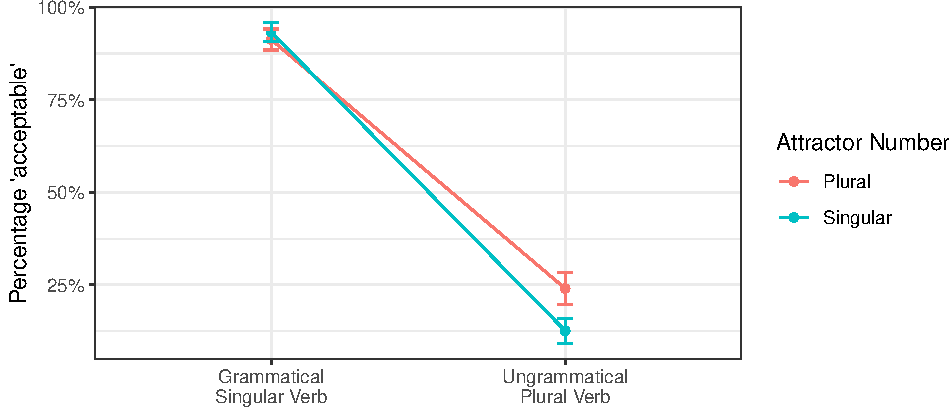
\includegraphics{paperdraft_files/figure-latex/UngBiasAvgResponse-1.pdf}
\caption{\label{fig:UngBiasAvgResponse}Experiment 1 Average Accuracy. Error bars are 95\% confidence intervals.}
\end{figure}

\begin{itemize}
\tightlist
\item
  The grammaticality status of the ungrammatical sentences with mismatching number are identified less easily than their matching counterpart.
\item
  The effect size is comparable to previous studies in Turkish (Lago et al., 2018; Türk \& Logačev, 2020): 0.11
\item
  No difference in accuracy between the grammatical conditions: 0.02.
\item
  Figure \ref{fig:UngBiasSubjDiff} shows the mean accuracy percentages and credible intervals by subject in ungrammatical conditions with a plural attractor.
\item
  It \emph{might} be a nice idea to include participant groups as a predictor in the model.
\item
  \textbf{Grammaticality assymetry still exists.}
\end{itemize}

\begin{figure}
\centering
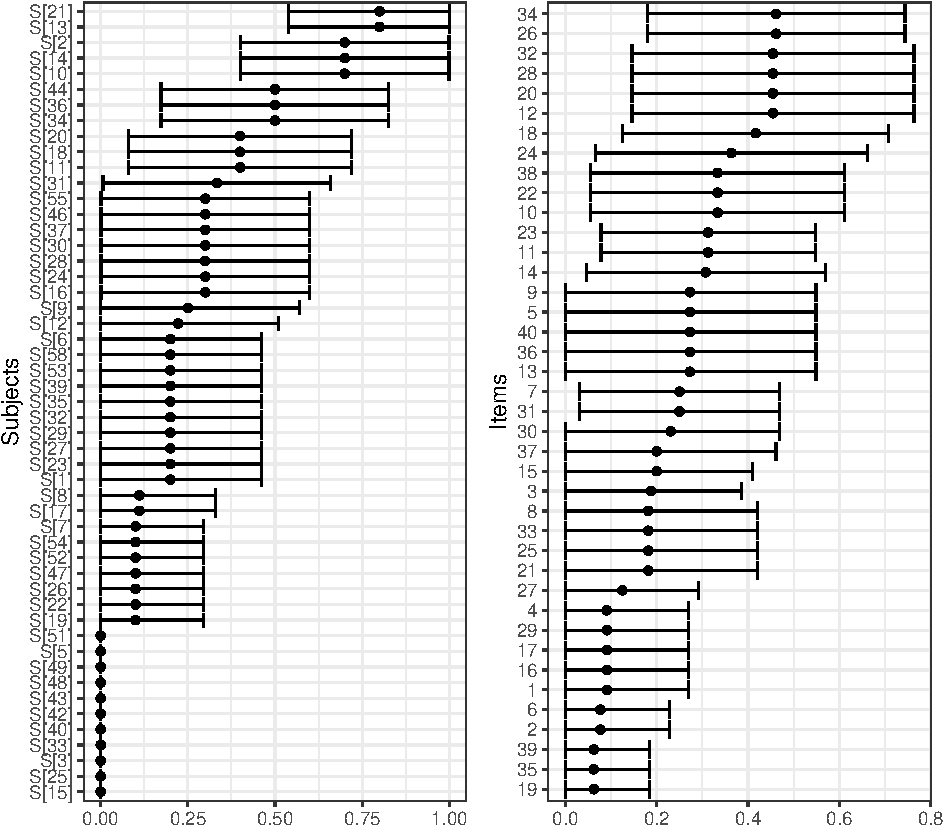
\includegraphics{paperdraft_files/figure-latex/UngBiasSubjDiff-1.pdf}
\caption{\label{fig:UngBiasSubjDiff}Subject Accuracy Averages and CIs}
\end{figure}

\hypertarget{modelling}{%
\subparagraph{Modelling}\label{modelling}}

\textbf{Model1}

\begin{figure}
\centering
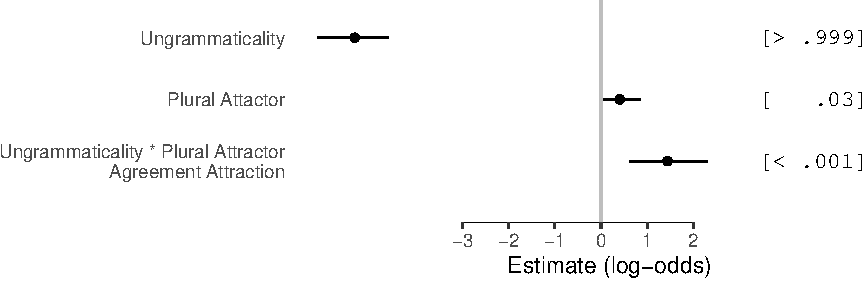
\includegraphics{paperdraft_files/figure-latex/Model1-1.pdf}
\caption{\label{fig:Model1}Estimates and 95\% credible intervals for the regression coefficients for the first model. Within-subject 95\% confidence intervals in brackets.}
\end{figure}

\begin{itemize}
\tightlist
\item
  The first model's estimates and 95\% credible intervals are shown in \ref{fig:Model1}.
\item
  Main \texttt{ungrammaticality} effect: \(\hat{\beta}=-5.33;\) \(CI=[-6.14; -4.61];\) \(P(\beta<0)> .999\). Participants may distinguish between ungrammatical and grammaticals.
\item
  Interaction effect: \(\hat{\beta}=1.44;\) \(CI=[0.62; 2.31];\) \(P(\beta<0)< .001\). Clear effect of agreement attraction.
\item
  Question from Utku: Where to look for the effect of attractor plural in grammatical sentences? Should the model be built differently?
\end{itemize}

\textbf{Model2}

\begin{figure}
\centering
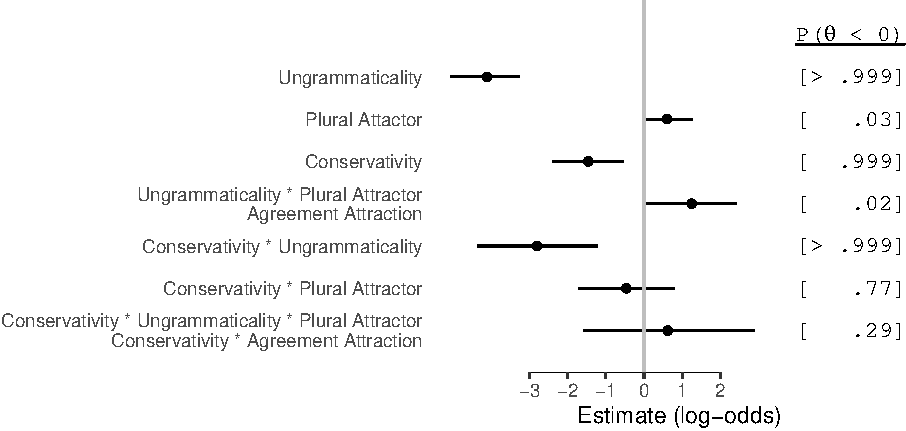
\includegraphics{paperdraft_files/figure-latex/Model1Grouped-1.pdf}
\caption{\label{fig:Model1Grouped}Estimates and 95\% credible intervals for the regression coefficients for the second model. Within-subject 95\% confidence intervals in brackets.}
\end{figure}

\begin{itemize}
\tightlist
\item
  The second model's estimates and 95\% credible intervals are shown in \ref{fig:Model1Grouped}.
\item
  Main \texttt{ungrammaticality} effect: \(\hat{\beta}=-4.11;\) \(CI=[-5.07; -3.26];\) \(P(\beta<0)> .999\). Participants may distinguish between ungrammatical and grammaticals.
\item
  Interaction effect: \(\hat{\beta}=1.24;\) \(CI=[0.06; 2.42];\) \(P(\beta<0)= .02\). Clear effect of agreement attraction.
\item
  It is clear that there is no different subject subgroups, at least the way I imagined them.
\end{itemize}

\hypertarget{rope-region-of-practical-equivalence}{%
\subparagraph{ROPE (Region of Practical Equivalence)}\label{rope-region-of-practical-equivalence}}

\begin{itemize}
\tightlist
\item
  hmm
\end{itemize}

\hypertarget{reading-times}{%
\paragraph{Reading Times}\label{reading-times}}

\begin{itemize}
\tightlist
\item
  hmm
\end{itemize}

\hypertarget{descriptive-1}{%
\subparagraph{Descriptive}\label{descriptive-1}}

\begin{itemize}
\tightlist
\item
  hmm
\end{itemize}

\hypertarget{modelling-1}{%
\subparagraph{Modelling}\label{modelling-1}}

\begin{itemize}
\tightlist
\item
  hmm
\end{itemize}

\hypertarget{rope-region-of-practical-equivalence-1}{%
\subparagraph{ROPE (Region of Practical Equivalence)}\label{rope-region-of-practical-equivalence-1}}

\begin{itemize}
\tightlist
\item
  hmm
\end{itemize}

\newpage

\hypertarget{experiment-2-grammatical-bias}{%
\subsection{Experiment 2: Grammatical Bias}\label{experiment-2-grammatical-bias}}

\begin{itemize}
\tightlist
\item
  Our experiments are located in this link: \url{}.
\end{itemize}

\hypertarget{methodology-1}{%
\subsubsection{Methodology}\label{methodology-1}}

I report how I determined our sample size, all data exclusions (if any), all manipulations, and all measures in the study.

\hypertarget{participants-1}{%
\paragraph{Participants}\label{participants-1}}

\begin{itemize}
\tightlist
\item
  I recruited total number of 56 students from the Department of Linguistics at Boğaziçi University.
\item
  I have excluded 5 of them due to their poor (below 60\%) score in the practice items.
\item
  The average age of the participants is 20.22.
\item
  Experiment were carried out following the Declaration of Helsinki and the regulations concerning ethics at research in Bo\u{g}azi\c{c}i University. All participants provided informed consent prior to their participation.
\end{itemize}

\hypertarget{materials}{%
\paragraph{Materials}\label{materials}}

\begin{itemize}
\tightlist
\item
  Same materials with the Experiment 1 were used.
\item
  Reverse distribution to the grammatical and ungrammatical filler sentences were assigned.
\item
  We have used 40 out of 60 filler items from the norming study. 10 of them were ungrammatical and 30 of them were grammatical.
\item
  The selection between the ungrammatical filler items made according to norming study results. We have selected 10 items that were found to be least acceptable.
\item
  The verb in grammatical fillers is always plural.
\item
  One group of the grammatical fillers (\(N=20\)) follows this template: \newline \emph{$\emptyset$ - [\textsubscript{Advcl} NP\textsubscript{\textsc{gen}}-NP\textsubscript{\textsc{poss}}-Adjunct-EmbeddedVerb ] -Verb}.
\item
  The first two NPs form the subject phrase of the adverbial clause, and the matrix verb is saturated by a pro-dropped subject argument.
\item
  The other group of the grammatical fillers (\(N=10\)) does not follow any template.
\item
  The verb in ungrammatical fillers is always singular.
\item
  A subset of the ungrammatical fillers (\(N=8\)) follows this template: \newline \emph{NP\textsubscript{\textsc{gen}}-NP\textsubscript{\textsc{poss}}-EmbeddedVerb ]-NP\textsubscript{\textsc{bare}}-Adjunct-Verb}
\item
  The ungrammaticality is a result of the mismatch between the voice of the matrix verb and the morphology of the NP\textsubscript{\textsc{bare}}. Since the voice of the sentences are active and the NP\textsubscript{\textsc{bare}} is not in the immediately preverbal position, NP must have been marked with an accusative case.
\item
  The rest of the ungrammatical fillers (\(N=2\)) does not follow a template.
\end{itemize}

\hypertarget{procedure-1}{%
\paragraph{Procedure}\label{procedure-1}}

\begin{itemize}
\tightlist
\item
  Same as the Experiment 1.
\item
  Only difference: Bias instruction.
\item
  They have been told that``Bu deneydeki cümlelerin ÇOĞU Türkçe kurallarına UYMAKTADIR!''
\item
  Translation: ``MOST of the sentences in this experiment DO COMFORT to Turkish grammar rules.''
\end{itemize}

\hypertarget{predictions-1}{%
\paragraph{Predictions}\label{predictions-1}}

\begin{itemize}
\tightlist
\item
  hmm
\end{itemize}

\hypertarget{analysis-1}{%
\paragraph{Analysis}\label{analysis-1}}

\begin{itemize}
\tightlist
\item
  hmm
\end{itemize}

\hypertarget{results-1}{%
\subsubsection{Results}\label{results-1}}

\begin{itemize}
\tightlist
\item
  hmm
\end{itemize}

\hypertarget{yes-responses-1}{%
\paragraph{Yes-Responses}\label{yes-responses-1}}

\begin{itemize}
\tightlist
\item
  hmm
\end{itemize}

\hypertarget{descriptive-2}{%
\subparagraph{Descriptive}\label{descriptive-2}}

\begin{itemize}
\item
  Seen in Figure \ref{fig:GBiasAvgResponse}

  \begin{itemize}
  \item
    mismatch and ungrammatical: (M = 0.11, SE = 0.02)
  \item
    match and ungrammatical: (M = 0.06, SE = 0.01)
  \item
    mismatch and grammatical: (M = 0.89, SE = 0.02)
  \item
    match and grammatical: (M = 0.94, SE = 0.01)
  \item
    ungrammatical filler sentences: (M = 0.07, SE = 0.01)
  \item
    grammatical filler sentences: (M = 0.89, SE = 0.01)
  \end{itemize}
\end{itemize}

\begin{figure}
\centering
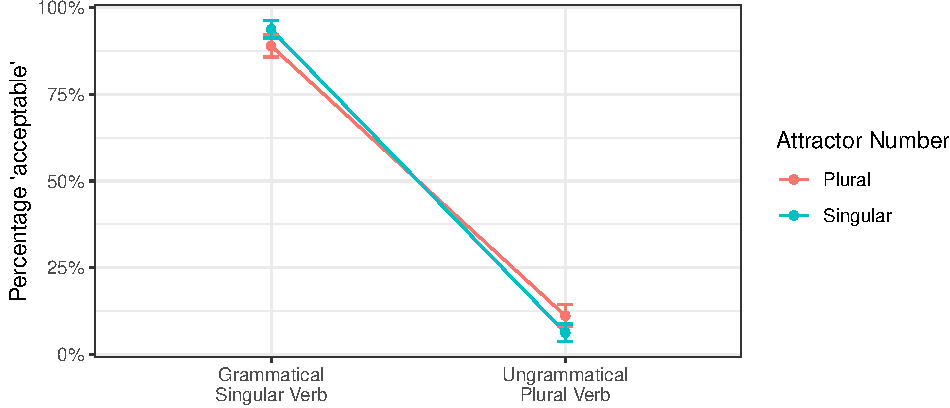
\includegraphics{paperdraft_files/figure-latex/GBiasAvgResponse-1.pdf}
\caption{\label{fig:GBiasAvgResponse}Experiment 1 Average Acceptability}
\end{figure}

\begin{itemize}
\tightlist
\item
  Ungrammatical sentences with mismatching head and attractor are more often identified correctly than their matching counterpart on average. However, the difference between them is not substantial.
\item
  The effect size is not comparable to previous studies in Turkish (Lago et al., 2018; Türk \& Logačev, 2020): -0.05
\item
  The effect size is substantially smaller than the Experiment 1: -0.07
\item
  The difference in accuracy between the grammatical conditions is really close to the that of ungramatical items: 0.02.
\item
  Figure \ref{fig:GBiasSubjDiff} shows the mean acceptability percentages and credible intervals by subject in ungrammatical conditions with a plural attractor.
\item
  By subject graphy looks closer to a simulated one. So, the variance is quite expected.
\item
  \textbf{Grammaticality assymetry still exists.}
\end{itemize}

\begin{figure}
\centering
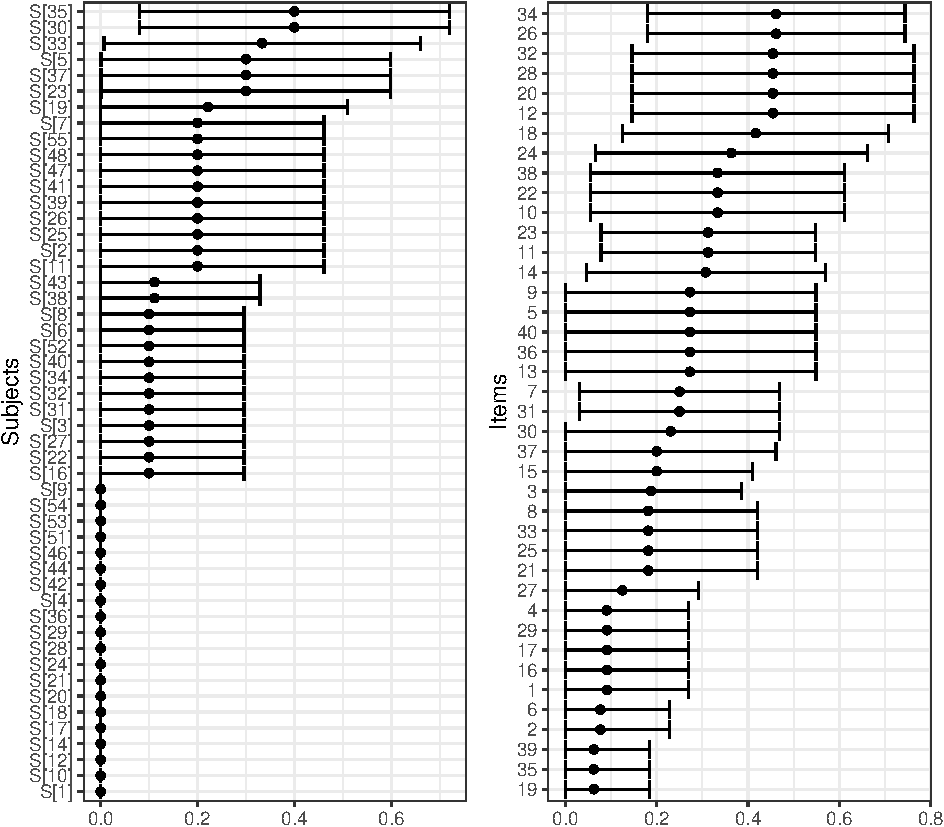
\includegraphics{paperdraft_files/figure-latex/GBiasSubjDiff-1.pdf}
\caption{\label{fig:GBiasSubjDiff}Subject Averages and CIs}
\end{figure}

\hypertarget{modelling-2}{%
\subparagraph{Modelling}\label{modelling-2}}

\begin{figure}
\centering
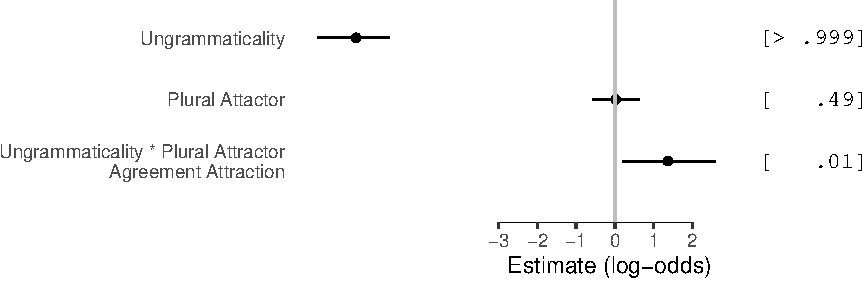
\includegraphics{paperdraft_files/figure-latex/Model2-1.pdf}
\caption{\label{fig:Model2}Estimates and 95\% credible intervals for the regression coefficients for the first model. Within-subject 95\% confidence intervals in brackets.}
\end{figure}

\begin{itemize}
\tightlist
\item
  The first model's estimates and 95\% credible intervals are shown in \ref{fig:Model2}.
\item
  Main \texttt{ungrammaticality} effect: \(\hat{\beta}=-6.67;\) \(CI=[-7.67; -5.80];\) \(P(\beta<0)> .999\). Participants may distinguish between ungrammatical and grammaticals.
\item
  Interaction effect: \(\hat{\beta}=1.36;\) \(CI=[0.20; 2.60];\) \(P(\beta<0)= .01\). Clear effect of agreement attraction.
\end{itemize}

\hypertarget{rope-region-of-practical-equivalence-2}{%
\subparagraph{ROPE (Region of Practical Equivalence)}\label{rope-region-of-practical-equivalence-2}}

\begin{itemize}
\tightlist
\item
  hmm
\end{itemize}

\hypertarget{reading-times-1}{%
\paragraph{Reading Times}\label{reading-times-1}}

\begin{itemize}
\tightlist
\item
  hmm
\end{itemize}

\hypertarget{descriptive-3}{%
\subparagraph{Descriptive}\label{descriptive-3}}

\begin{itemize}
\tightlist
\item
  hmm
\end{itemize}

\hypertarget{modelling-3}{%
\subparagraph{Modelling}\label{modelling-3}}

\begin{itemize}
\tightlist
\item
  hmm
\end{itemize}

\hypertarget{rope-region-of-practical-equivalence-3}{%
\subparagraph{ROPE (Region of Practical Equivalence)}\label{rope-region-of-practical-equivalence-3}}

\begin{itemize}
\tightlist
\item
  hmm
\end{itemize}

\hypertarget{discussion}{%
\subsection{Discussion}\label{discussion}}

\begin{itemize}
\tightlist
\item
  Write here some stuff that what we have expected and how it is not we found at all.
\item
  So, maybe we should check for bias and group people according to the bias.
\item
  Our manipulation may
\end{itemize}

\newpage

\hypertarget{chapter-6-post-hoc-bias-analysis}{%
\section{Chapter 6: Post-Hoc Bias Analysis}\label{chapter-6-post-hoc-bias-analysis}}

\begin{itemize}
\tightlist
\item
  Following Macmillan and Creelman (2005), we calculate \emph{c} values of the participants.
\item
  Formula used is as the following:
\end{itemize}

\(c = - \frac{Z(Hit\ Rate)\ +\ Z(False\ Alarm\ Rate)}{2}\)

\begin{itemize}
\item
  Negative c implies bias towards grammatical responses.
\item
  Positive c implies bias towards ungrammatical responses.
\item
  The main point in Hammerly, Staub, and Dillon (2019) was that in the experiment with no manipulation the \emph{c} value was negative and participants were biased towards grammatical responses.
\item
  With their manipulations, they had average \emph{c} values that are mainly centered around zero.
\item
  In this work, we will use the same formula for calculating \emph{c} values and the same code that Hammerly, Staub, and Dillon (2019) used.
\item
  However, unlike Hammerly et al., we will use only the filler items for the calculation. The reason behind this is that using experimental items in \emph{c} value calculation will create a confound where the \emph{c} values are affected by the degree of agreement attraction and all becomes circular.
\item
  After cutting the cake as people with grammatical and ungrammatical response bias, we plotted the descriptive stats to have a general picture.
\item
  Lastly, we fitted a model where we included the predictors for the categorical bias, grammaticality, and plural attractor.
\end{itemize}

\hypertarget{bias-distribution-within-experiments}{%
\subsection{Bias Distribution within Experiments}\label{bias-distribution-within-experiments}}

\begin{itemize}
\tightlist
\item
  Within our experiments, it is possible that we have failed the manipulate bias of the participants uniformly.
\item
  In order to check it, we have calculated the bias within our experiments.
\item
  Figure \ref{fig:Biasbyexperiment} shows that participants with both positive and negative \emph{c}-values can be found in either of the experiments.
\item
  From now on, we calculate the RTs and percentage of \emph{yes} responses according to the grouping based on c-value.
\item
  This will help us test whether or not we were able to replicate the predictions of the diffusion model.
\end{itemize}

\begin{figure}
\centering
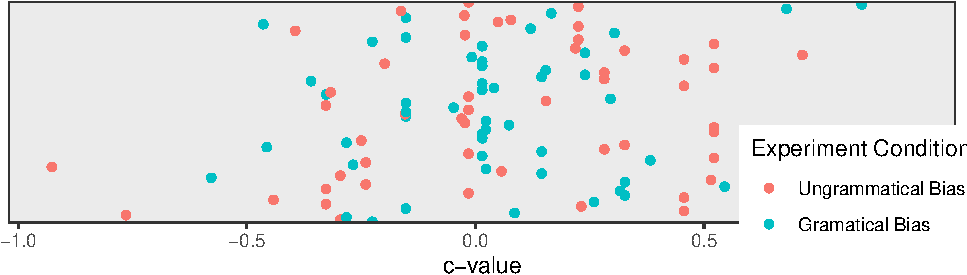
\includegraphics{paperdraft_files/figure-latex/Biasbyexperiment-1.pdf}
\caption{\label{fig:Biasbyexperiment}Estimates and 95\% credible intervals for the regression coefficients for the first model. Within-subject 95\% confidence intervals in brackets.}
\end{figure}

\begin{itemize}
\tightlist
\item
  In our experiments, it first seemed like bias manipulation did not really matter for agreement attraction as previously suggested by Hammerly, Staub, and Dillon (2019).
\item
  When looked at closely, we have seen that our manipulations did not align with the overall bias within the experiments. This means that participants in our experiments were not grouped within positive or negative \emph{c}-values.
\item
  Instead, they were all grouped around \emph{c}-value \(0\) regardless of our manipulation.
\item
  Seeing this failure of manipulation, we grouped participants according to their \emph{c}-values.
\item
  Our expectation is that when people have a positive \emph{c}-value, they are biased towards ungrammatical responses. Therefore, their reading times in grammatical conditions will be slightly longer than the ones that are biased towards grammatical responses. This result is the direct result of diffusion model.
\item
  In addition, participants biased towards ungrammatical response should deem grammatical sentence ungramatical more often than the participants who are biased towards grammatical. This also follows the assumption of the diffusion model.
\item
  For our purposes, what is interesting is that the illusion of ungrammaticality and the effect of plural attractor in this illusion.
\item
  Following the assumptions of Marking and Morphing combined with the diffusion model decision making, we would predict that similar to grammaticality illusion, people that are biased towards ungrammatical responses should also exhibit ungrammaticality illusion. And, similar to the case in grammaticality illusion, the magnituted of ungrammaticality illusion should also differ according to the existence of plural attractor.
\item
  That is, we expect when there is a plural attractor, people should do more errors in judging the sentence's grammaticality correctly regardless of sentence's grammaticality.
\end{itemize}

\hypertarget{yes-responses-2}{%
\subsection{Yes-Responses}\label{yes-responses-2}}

\begin{itemize}
\tightlist
\item
  hmm
\end{itemize}

\hypertarget{descriptive-look}{%
\subsubsection{Descriptive Look}\label{descriptive-look}}

\begin{itemize}
\tightlist
\item
  Figure \ref{fig:BeforeBiasDivide} shows the picture prior to our division with bias values. As it can be seen from the data, it seems like participants who that are intended to be biased towards ungrammatical responses do not show agreement attraction effects. Surprisingly, they accepted sentences with a plural attractors less often as acceptable sentences than the ones with a singular attractor when the sentence is grammatical. This finding is completely unexpected in any theoretical explanation of agreement attraction.
\end{itemize}

\begin{figure}
\centering
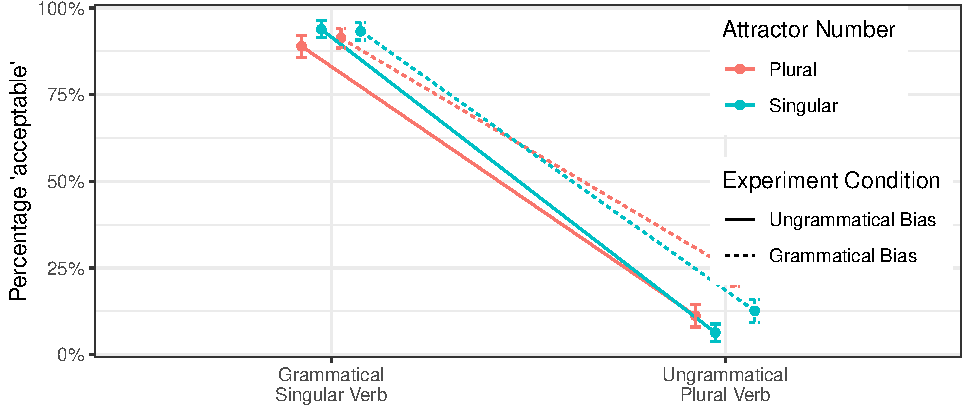
\includegraphics{paperdraft_files/figure-latex/BeforeBiasDivide-1.pdf}
\caption{\label{fig:BeforeBiasDivide}Percentage averages of yes responses. Solid lines represents grouping according to our bias manipulation while the color represents the attractor number. Error bars represents the standard error.}
\end{figure}

\begin{itemize}
\tightlist
\item
  When we group according to the bias, the data seems more reasonable.
\item
  Figure \ref{fig:UngBiasResponse} shows us that people make errors in judgment more often when the attractor is plural regardless of the grammaticality of the verb. And the difference in grammatical and ungrammatical sentences is substantial, meaning that error bars do not overlap.
\item
  Another thing that is interesting about this graph is that the magnitude of agreement attraction effect is lower than the previous studies in Turkish. We see that the difference within ungrammatical sentences is 0.06\%. Previous experiments in Lago et al. (2018) and Türk and Logačev (2020) found the magnitude around 11\%.
\end{itemize}

\begin{figure}
\centering
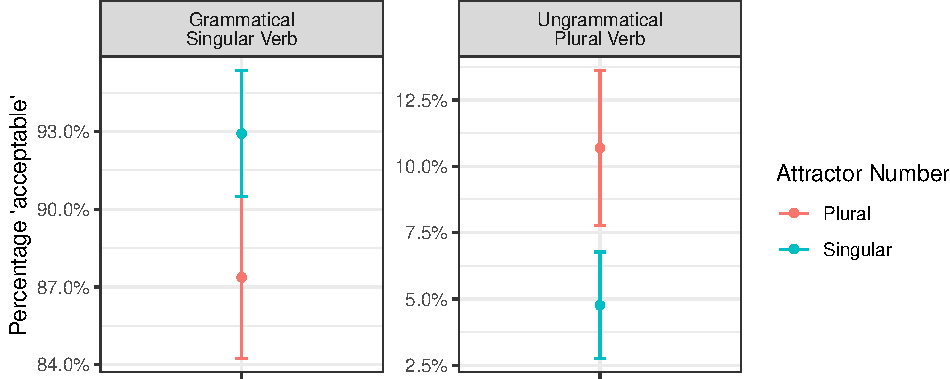
\includegraphics{paperdraft_files/figure-latex/UngBiasResponse-1.pdf}
\caption{\label{fig:UngBiasResponse}Percentage averages of yes responses of participants with positive c-value. Error bars represents the standard error.}
\end{figure}

\begin{itemize}
\tightlist
\item
  Contrary to what we see in Figure \ref{fig:UngBiasResponse}, in Figure \ref{fig:GBiasResponse} we see that participants that are biased towards grammatical responses only make additional grammaticality judgment mistakes in ungrammatical sentences. This phenomenon is known as grammaticality asymmetry.
\item
  Similar percentages of acceptable responses within grammatical conditions are expected if the participants are biased towards grammatical responses.
\item
  Expectedly, the magnitude of agreement attraction within ungrammatical sentences is comparable to previous agreement attraction experiments in Turkish: 0.11\%
\end{itemize}

\begin{figure}
\centering
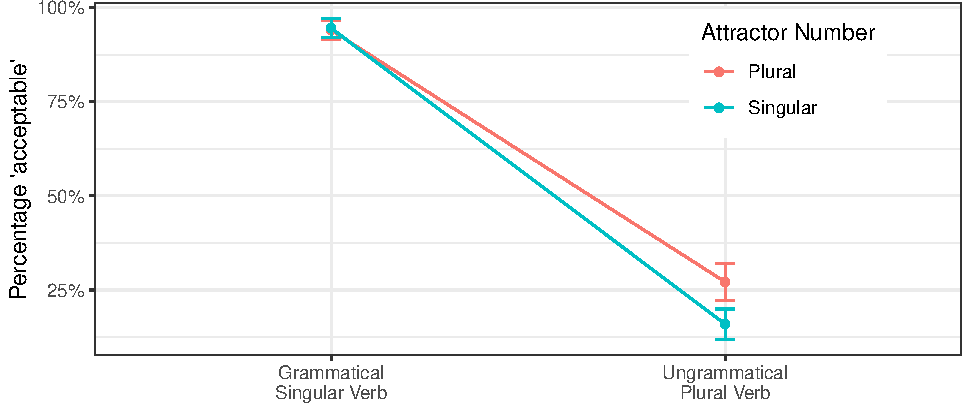
\includegraphics{paperdraft_files/figure-latex/GBiasResponse-1.pdf}
\caption{\label{fig:GBiasResponse}Percentage averages of yes responses of participants with positive c-value. Error bars represents the standard error.}
\end{figure}

\begin{itemize}
\tightlist
\item
  When grouped according to their c-values, percentage of yes responses becomes meaningful.
\end{itemize}

\hypertarget{modelling-yes-responses}{%
\subsubsection{Modelling Yes-Responses}\label{modelling-yes-responses}}

\begin{itemize}
\item
  For more interference on responses, we have fitted a maximal model that uses following predictors and contrasts given in parentheses:

  \begin{itemize}
  \tightlist
  \item
    our intended bias manipulation (\texttt{0.5} for intended grammatical and \texttt{-0.5} intended ungrammatical),
  \item
    categorical version of calculated bias of the participants (\texttt{0.5} for bias towards grammatical and\texttt{-0.5} for ungrammatical),
  \item
    attractor number (\texttt{0.5} for plural and \texttt{-0.5} for singular)
  \item
    ungrammaticality of the sentence (\texttt{0.5} for ungrammatical, \texttt{-0.5} for grammatical)
  \item
    and their interactions.
  \end{itemize}
\item
  Additionally, we have included random slopes for ungrammaticality and plural attractor predictors for participants and random slopes for bias, ungrammaticality and plural attractor predictors for items.
\item
  Our model also includes random intercepts for participants and items.
\item
  In this model, we are using defaults priors from \texttt{brms} package.
\item
  The formula used within \texttt{brm} function of \texttt{brms} package:
\end{itemize}

\begin{verbatim}
response_yes ~  cBias * cExp * cUngrammatical * cAttractorPlural +
                (cUngrammatical * cAttractorPlural + 1| subject) +
                (cBias * cUngrammatical * cAttractorPlural + 1| item)
\end{verbatim}

\begin{figure}
\centering
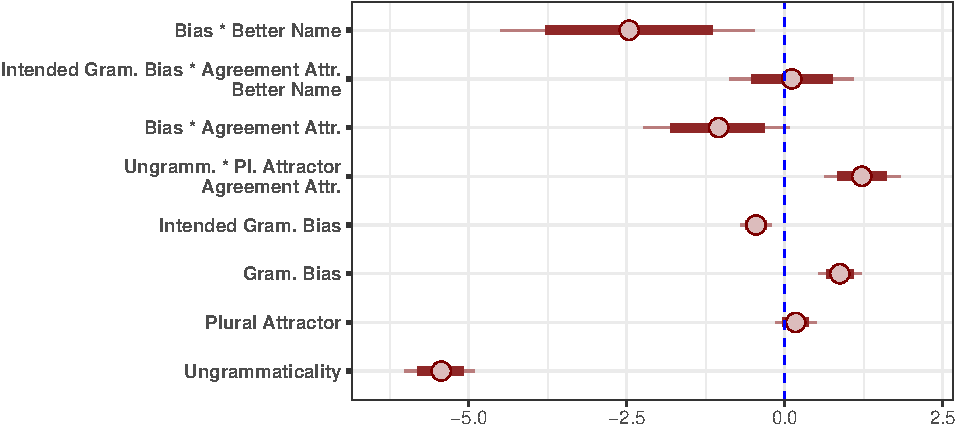
\includegraphics{paperdraft_files/figure-latex/BiasModelCoefPlot-1.pdf}
\caption{\label{fig:BiasModelCoefPlot}Uncertainty intervals computed from posterior draws for selected coefficients. The estimate shown as point is the median value of the draws. The bold interval signifies the probability mass of 80\%. The slim tails represents the probability mass from 80 to 95\%.}
\end{figure}

\begin{itemize}
\item
  The estimates from the certain coefficients of the model in Figure \ref{fig:BiasModelCoefPlot} tells us that participants responses with less yes responses when the sentences were ungrammatical.
\item
  While people real grammatical bias gave more yes responses overall, our intended grammatical bias manipulation did the reverse effect.
\item
  In average, people showed agreement attraction effects, that is they gave more yes-responses when sentences were ungrammatical and there was a plural attractor.
\item
  Our manipulation of grammatical bias seems to be not effective. The uncertainty intervals contains zero and the most of the mass is centered around the zero.
\item
  It seems that real grammatical bias, on the other hand, affected agreement attraction within ungrammatical sentences negatively. People with negative \emph{c}-values gave yes responses less often compared to people with positive \emph{c}-values when the sentence is ungrammatical and there is a plural attractor.
\item
  Questions:

  \begin{itemize}
  \tightlist
  \item
    how can I talk about the ungrammaticality illusion with this model?
  \item
    What does it mean to have 4-way interaction? Something in the lines of: Our experimental manipulation worked better in catalizing agreement attraction effects when people were already biased?
  \end{itemize}
\end{itemize}

\hypertarget{rope-region-of-practical-equivalence-4}{%
\subsubsection{ROPE (Region of Practical Equivalence)}\label{rope-region-of-practical-equivalence-4}}

\begin{itemize}
\tightlist
\item
  hmm
\end{itemize}

\hypertarget{reading-times-2}{%
\subsection{Reading Times}\label{reading-times-2}}

\begin{itemize}
\tightlist
\item
  hmm
\end{itemize}

\hypertarget{descriptive-4}{%
\subsubsection{Descriptive}\label{descriptive-4}}

\begin{itemize}
\tightlist
\item
  hmm
\end{itemize}

\hypertarget{modelling-4}{%
\subsubsection{Modelling}\label{modelling-4}}

\begin{itemize}
\tightlist
\item
  hmm
\end{itemize}

\hypertarget{rope-region-of-practical-equivalence-5}{%
\subsubsection{ROPE (Region of Practical Equivalence)}\label{rope-region-of-practical-equivalence-5}}

\begin{itemize}
\tightlist
\item
  hmm
\end{itemize}

\hypertarget{discussion-1}{%
\subsection{Discussion}\label{discussion-1}}

\begin{itemize}
\tightlist
\item
  hmm
\end{itemize}

\hypertarget{chapter-7-conclusion}{%
\section{Chapter 7: Conclusion}\label{chapter-7-conclusion}}

\begin{itemize}
\tightlist
\item
  hmm
\end{itemize}

\newpage

\hypertarget{references}{%
\section{References}\label{references}}

\begingroup
\setlength{\parindent}{-0.5in}
\setlength{\leftskip}{0.5in}

\hypertarget{refs}{}
\begin{CSLReferences}{1}{0}
\leavevmode\hypertarget{ref-HammerlyEtAl2019}{}%
Hammerly, C., Staub, A., \& Dillon, B. (2019). The grammaticality asymmetry in agreement attraction reflects response bias: Experimental and modeling evidence. \emph{Cognitive Psychology}, \emph{110}(January), 70--104. \url{https://doi.org/10.1016/j.cogpsych.2019.01.001}

\leavevmode\hypertarget{ref-LagoEtAl2018}{}%
Lago, S., Felser, C., Gračanin-Yuksek, M., Demir, O., Kırkıcı, B., \& Şafak, D. F. (2018). Straight from the horse's mouth: Agreement attraction effects with Turkish possessors. \emph{Linguistic Approaches to Bilingualism}, \emph{12}(1), 1--29. \url{https://doi.org/10.1075/lab.17019.lag}

\leavevmode\hypertarget{ref-MacmillanCreelman2005}{}%
Macmillan, N. A., \& Creelman, C. D. (2005). \emph{Detection Theory (2nd edition)}. Mahwah, NJ: Erlbaum.

\leavevmode\hypertarget{ref-TurkLogacev2020}{}%
Türk, U., \& Logačev, P. (2020). \emph{The role of shallow processing in agreement attraction}. Amherst, MA. Retrieved from \url{https://osf.io/x9pv7/}

\end{CSLReferences}

\endgroup


\end{document}
